%%%%%%%%%%%%%%%%%%%%%%%%%%%%%%%%%%%%%%%%%%%%%%%%
%
% Strath PhD Thesis Template
%	by Jethro Browell [jethro.browell@strath.ac.uk]
%
%	Guidelines for thesis format, submission and content are found in
%	General and Course Regulations for Graduate and Postgraduate
%	Awards and Degrees, section 20.6.
%
%	Using .eps or .pdf is recomended to prduce high quality figures etc.
%
%	The Strathclyde logo can be found in other formats at www.strath.ac.uk.
%
%%%%%%%%%%%%%%%%%%%%%%%%%%%%%%%%%%%%%%%%%%%%%%%%

\documentclass[a4paper,oneside,11pt]{book}
\setcounter{secnumdepth}{3}
\usepackage{amsbsy}
\usepackage{amsmath}
\usepackage{amsfonts}
\usepackage{graphicx}
\usepackage{multirow}
\usepackage{mathrsfs}
\usepackage{color}
\usepackage[hidelinks]{hyperref}
\usepackage{cite}
\usepackage{enumitem}
\usepackage{epsfig}
\usepackage{caption}
\usepackage{subcaption}
\usepackage[strict]{changepage}

% Page Margins - Strath Requirement
\usepackage[left=4cm,right=2.5cm,top=2cm,bottom=4cm,includehead,includefoot,headheight=15pt]{geometry}

% Page Headers
\usepackage{fancyhdr}
\fancyhf{}
\renewcommand{\headrulewidth}{0pt} % optional
%\fancyhead[L]{\nouppercase{\leftmark} \hfill Section \nouppercase{\rightmark}}
\fancyhead[L]{\nouppercase{\leftmark}}
\cfoot{\thepage}
\pagestyle{fancy}

% Draft Watermark
\usepackage[draft=true,allpages=true,fontfamily=cmr,angle=90,scale=0.1,mark={\fboxsep=35pt\fboxrule=0pt\relax\fbox{-- DRAFT -- \today~--}},xcoord=-80,ycoord=-20]{draftmark}


% Line Spacing
%\def\baselinestretch{1.5} 
\usepackage{setspace}
\setstretch{1.5}


% Place UoS Logo on Title Page (this package modifies the "\maketitel" command.)
\usepackage{titling}


%%%%%%%%%%%%%%%%%%%%%%%%%%%%%%%%%%%%%%%%%%%%%%%%%%%%%%%%%%%%%%
\begin{document}
%%%%%%%%%%%%%%%%%%%%%%%%%%%%%%%%%%%%%%%%%%%%%%%%%%%%%%%%%%%%%%

\setcounter{chapter}{4}
\chapter{Detection and Characterisation of rotational spherical aggregate rotational dynamics}
\section{Simulative QPD}
A QPD is simply a measure of the total electric field incident on a photo diode, in order to accurately simulate a QPD response careful consideration of how the Electromagnetic fields are defined is required. 

\subsection{Incident beam}
\label{sec:scattering}
The incident beam is simple enough to define given our set up parameters, for the sake of simplicity we assume that our beam is a Laguerre-Gaussian beam of mode $[0.0, 0.0]$ (which is simply a pure Gaussian beam). *Ott* uses a point matching approach to approximate the beam shape coefficients of the incident field by fitting it to the far field estimate, the beam is of the form:

\begin{align}
	E_{inc}(kr)=\sum^\infty_n\sum^n_{m=-n}a_{mn}RgM_{nm}(kr)+b_{nm}RgN_{nm}(kr)
\end{align}

Where $RgM_{nm}(kr)$ \& $RgN_{nm}(kr)$ are regular vector spherical wave functions, *ott* allows us to change the basis of the the incident beam to suit our needs, because we are measuring in the far field we want to set our incident beam to be an outgoing spherical wave so that we can compute the intensity on the QPD. For spherical waves the field can either be expressed as an incoming/outgoing wave (with a singularity at the origin) or as a regular wave around the origin; for incoming/outgoing waves the wave functions use the first/second forms of the Hankel function respectfully. In order to compute the regular spherical wave at the origin we replace the Hankel function with the Bessel function which is simply the average of the first and second forms of the Hankel function, so at the origin we avoid a singularity of the EM field.  

We can if we want further restrict the incident beam by applying setting the truncation angle to match our microscope object, this essentially applies a cut off point to the In order to compute the scattering from the target particle *ott* uses the t-matrix method, this is not essential for a simple sphere but is far more important for complex shaped particles such as our dimers. If the T-matrix is loaded in from *mstm* we need to convert the *mstm* t-matrix to a form more suitable for *ott*:

\begin{align}
	\begin{pmatrix}
		p_{nm}\\
		q_{nm}
	\end{pmatrix} =T 
	\begin{pmatrix}
		a_{nm}\\
		b_{nm}
	\end{pmatrix} = 
	\begin{pmatrix}
		aT^{TM}_{nm} & aT^{TE}_{nm}\\ 
		bT^{TM}_{nm} & bT^{TE}_{nm}
	\end{pmatrix}
	\begin{pmatrix}
		a_{nm}\\
		b_{nm}
	\end{pmatrix}
\end{align} 

For *mstm* the T-matrix is packed as a column vector:

\begin{align}
	T_{MSTM} = 
	\begin{bmatrix} 
		aT^{TE}_{n,-n} & bT^{TE}_{n,-n} \\ 
		aT^{TE}_{n, -n+1} & bT^{TE}_{n, -n+1} \\ 
		... & ...\\ 
		aT^{TE}_{n,n} & bT^{TE}_{n,n} \\ 
		----&----\\ 
		bT^{TM}_{n,-n} &bT^{TM}_{n,-n} 
	\end{bmatrix}
\end{align}

Where as *ott* packs packs the T-matrix with sub matrices:

\begin{align}
	T_{Ott} = 
	\begin{bmatrix} 
		\begin{pmatrix}
			aT^{TM}_{n,-n} & aT^{TE}_{n,-n}\\ 
			bT^{TM}_{n,-n}&bT^{TE}_{n,-n}
		\end{pmatrix} \\ 
		\begin{pmatrix}
			aT^{TM}_{n,-n+1} & aT^{TE}_{n,-n+1}\\ 
			bT^{TM}_{n,-n+1} & bT^{TE}_{n,-n+1}
		\end{pmatrix}\\
		....\\ 
		\begin{pmatrix}
			aT^{TM}_{nm} & aT^{TE}_{nm}\\ 
			bT^{TM}_{nm} & bT^{TE}_{nm}
		\end{pmatrix}
	\end{bmatrix}
\end{align}

\subsection{Scattered and Total Fields}
With the T-matrix in hand we can compute the scattered beam by multiplying our beam shape coefficients with the T-matrix to get out the scattered field. Now in order to simulate a real QPD we need to account for the motion of our target particle within the trap, taking a typical trajectory file we read off each line in order to translate and rotate the beam. Translation is a rather simple process, simply involving us to shift the beam laterally, small deflections are generally unnoticeable for the incident beam but are much more noticeable in the scattered field (the below figure shows the result of shifting the incident beam $1\mu m$ to the right):

The QPD does not just pick up the scattered light however, it instead is receiving a combined signal from both the incident field and scattered field simultaneously, as mentioned by \textcolor{red}{Rohrbach} the total intensity can be computed by taking the magnitude of both the incident field *focused at the origin $[0,0,0]$* and the scattered field originating from $[\delta x, \delta y, \delta z]$ (top left and bottom right plots in the above figure). This means we do not need to worry about any translation effects being 'double-counted' in the QPD's signal as we are only shifting the scattered field meaning the QPD signal is only picking up the interference due to the shifted scattered field. I conducted some unitary tests where I scanned the beam position laterally along the x-axis and measured the QPD's 'x-signal' for x, circular and y-polarized light which yielded the following QPD responses. The target particle was $1.57\ \mu m$ and the scan range is set to $[-4, 4 \mu m]$

Where $S_x$ is given in blue, and $S_y$ is given in orange, the plots make it clear that the polarisation of the beam have a minimal effect on the QPD signals if the particle is traversing in one direction, its clear that the displacement from the beam centre is far more important than the polarization of said beam. This is backed up when we look at \textcolor{red}{Rohrbach's} results, who studied a $150\ nm$ sphere ($n=1.57$) submerged in water with a focusing lens of numerical aperture 1.2, and beam power of $3\ mW$. The condensing lens' numerical aperture was not set to a particular value and was instead varied between 0.13-1.2, as a compromise we selected a condenser numerical aperture of 0.525, corresponding to a acceptance angle of $31.6^\circ$. 

Where the points are Rohrbach's results and the solid line's are our QPD's own replication. The dashed horizontal lines on the left represent the maximum displacement in the lateral displacement which is given by the combined beam radius and particle radius (assuming a beam radius of $0.54\ \mu m$); we can say that any displacements beyond this distance, while non-zero these displacements are unlikely to occur while a particle is trapped at the focus. Whereas the right most plot's dashed horizontal lines represents the Rayleigh range of the Gaussian beam, this represents the transition between plane wave and spherical wave regimes. Interestingly while our results close to Rohrbach's while close to the focus we see it begins to diverge beyond the first peak, this shouldn't be an issue for a typical optical tweezer calibration as we can assume that the maximum displacement will be within this linear regime. 

Now the above plots only consider the QPD response to movements along the cartesian axis, however obviously for any Brownian motion the movements are a combination of displacements in each cartesian direction. We might assume naively that any displacement $\Delta r$ will result in a linear combination of QPD responses; for low precision force measurements this assumption is adequate, however when high precision is required we find that this assumption is longer adequate due to something referred to as cross-talk. Cross talk arises when movement in one direction results in a QPD response change in the other orthogonal direction, there is no one reason for this effect, it could be a result of differing sensitivity in the photo diodes, it could be because the scattering is slightly asymmetric meaning the scattering falls outside the QPD, or it could be a result of mis-alignment in the set up. This can have unintended effects, for example it may lead to the apparent rise of a curved trajectory rather than a straight path: Consider a particle moving purely along the x-axis, with 0 cross-talk the QPD response should perfectly match the above curve $S_x(x,0,z_0)$, with $S_y$ being flat in comparison; if however there is cross talk between the channels then $S_y$ will have some significant non-zero value (or it may even grow with increasing displacement), implying that the particle is actually moving in both the x and y directions simultaneously.  First we checked for this by measuring the QPD response for random positions within the XY plane:

Where $S_x$ is plotted on top and $S_y$ is plotted below, as shown by the above plot we see that they still possess similar shapes to the previous plots but now with additional noise terms, making it clear that for any trajectory there will be cross talk. This means that trying to get a one-to-one measurement of the particle's displacement is not possible by simply looking at the QPD response, to do that we can need to calibrate the trap. 

\textcolor{red}{Berg and Flyvbjerg} have an excellent breakdown for accurately calibrating an optical tweezer, in addition they discuss how to minimise cross-talk effects. For two correlated power spectra, the cross correlation is given as:

\begin{align}
	P_{x} = |\hat{S}_x(f)|^2 \\ 
	P_{y} = |\hat{S}_y(f)|^2 \\
	\rightarrow P_{xy} = Re(\hat{S}_x\hat{S}^*_y)
\end{align}

Now if the two directions are correlated then $|P_{xy}|^2/P_xP_y$  should be non-zero for all frequencies, in order to eliminate cross-talk effects we need to minimise the cross-correlation for all frequencies. They showed that it is possible to find a transformation of the time series $(x(t), y(t))$  to one that possesses the property that $P_{x'y'}(f)=0$ for all frequencies. They found these transformed positions by minimising the sum cross-correlation:

\begin{align}
	\sum\frac{P_{x'y'}}{P_{x'}P_{y'}} = \sum\frac{(1+bc)P_{xy}+cP_x+bP_y}{(P_x+2bP_{xy}+b^2P_y)(Py+2cP_{xy}+c^2P_y)}
\end{align}

Where b and c are fitting parameters, by minimising this function one can adjust each spectra in order to eliminate cross talk effects and provide a more accurate calibration of the optical trap. Furthermore with the fitting completed, the time series can be then transformed in order to eliminate the cross talk effects:

\begin{align}
	x'(t) = S_x(t) + bS_y(t),\ y'(t) = S_y(t) + cS_x(t)
\end{align}

Where $x'$ and $y'$ are now uncoupled coordinates that when Fourier transformed provide the uncorrelated power spectrum. With the fitting complete we can now adjust our time series in order to get a replication of the lateral trajectory. 

\section{Rotations and Asymmetric particles}
Rotational motion is something that is not often necessarily considered when characterising Brownian motion, often because separating the contributions from rotational and translational motion is challenging. Depending on the rotational and translational trap stiffness the collected QPD signal will be aliased and typical calibration techniques cannot characterise the particle and trap interactions. This is often why most of the research into trapping asymmetric objects does not delve into power spectra analysis, as there is no real way of modelling the QPD response from an asymmetric object. 

Now for isotropic scatterers any rotation is often not an issue when it comes to QPD analysis, even if a sphere rotates $180^{\circ}$the scattering should be identical (assuming its relative position is the same). Now *ott* deals with both translations and rotations by moving the beam itself and computing the scattering from by once again expanding the spherical wave functions, the problem that arises from this is that the portion of the spherical wave that is evaluated by the QPD will pick up said rotation and produce a non-zero signal even if the scatterer in question is isotropic. This means we need to counter rotate the total field prior to collecting the QPD signal, this captures the effects of an anisotropic scatterer but has no effect for an isotropic scatterer. As a test the QPD response from an isotropic sphere of $1.57 \ \mu m$ was collected at multiple angles, between 0 and $2\pi$, then as a comparison a symmetrical and 1:2 dimer were also subjected to the same rotations and their QPD responses evaluated. 

Where on the left we have an isotropic sphere, then a symmetrical dimer, and lastly a 1:2 dimer. The left most plot shows that simply using the inverted rotation matrix is sufficient to prevent rotation effects being double counted.
For dimers however, rotating about a given axis gives us a clear change in the signal for even a slight rotation about any axis. 

\section{Power Spectra of single sphere vs spherical aggregates}
In order to verify that the QPD is outputting correct signals we first compared the module to the only other known instance of simulating a QPD response, that being the work of \textcolor{red}{Rorhbach}. In their paper they looked at the signal response produced by a single sphere ($r = 150\ nm$, $n = 1.57$) being scanned along the three Cartesian axis in the proximity of a $1064\ nm$ NIR beam with a numerical aperture of 1.2. As shown by fig~\ref{fig:Rohrbach} the two responses are remarkably accurate close to the origin; with only slight deviations as you move past the harmonic region, the difference can be explained due to how the two evaluate the total fields. Where in our case the incident and scattered fields are reduced to 0 at the origin, whereas Rohrbach's work evaluates the fields the fields as being non-zero at all points, as you move beyond the origin this discrepancy grows. 

\begin{figure}[h]
	\label{fig:Rohrbach}
	\begin{subfigure}{0.475 \linewidth}
		\subcaption{}
		\includegraphics[width=\linewidth]{QPD_axial_tests.png}
	\end{subfigure}
	\begin{subfigure}{0.475 \linewidth}
		\subcaption{}
		\includegraphics[width=\linewidth]{QPD_lat_tests.png}
	\end{subfigure}
	\caption{Comparison between QPD response signal versus work conducted by Rohrbach, single sphere ($r = 150\ nm$, $n=1.57$) is scanned by a $1064\ nm$ laser and the QPD signal recorded. Solid lines represent the signal produced by QPD using \textit{ott} and points represent the signal response collected from [].}
\end{figure}
Since we are only interested in the dynamics of spherical aggregates upon reaching equilibrium we do not need to be concerned about the deviation from Rohrbach's results so long as the particle's displacement does not exceed the linear region at the origin. The axial response curve is slightly more involved, requiring that the condenser lens numerical aperture is adjusted until a harmonic response curve is achieved \cite{Friedrich2012}. 

In order to verify that the QPD can accurately capture the dynamics of the target particle we first simulated a single sphere ($a = 1\mu\ m$, $n=1.59$) in the focus of a $1064\ nm$ laser. Using \textit{ott} the trap stiffness is computed by applying a linear fit to the force-displacement curve along the x and y axis'; for a linearly polarised trap the gradient force is greater in the polarisation direction than transverse case. We see this reflected in the simulated QPD, the fitted Lorentzian curves have different corner frequencies indicating that the beam's polarisation is influencing the dynamics of the trap. 

Next we consider a dimer composed of two sphere's similar to the previous sphere, we again apply the QPD module to reproduce the power spectrum. Previous experimental work found that a pair of trapped beads would half the corner frequency from the reported power spectra. However, in our own simulations we see instead an increase in the expected trapping force from our QPD method, with the maximum trap stiffness expected for a dimer of size ratio 5. Compared to \textit{ott} in which the maximum trapping strength is expected at a size ratio of 2. This can be somewhat explained by the fact that as the second sphere shrinks the centre of diffusion approaches the centre of the larger sphere and thus the dimer's orientational behaviour is similar to a single sphere, only subject to slight Brownian motion. Therefore one should expect that for aggregates containing multiple sized particles (e.g. cellular samples) typical characterisation techniques may over estimate the strength of the trap.

Now one of the things that has yet to be covered in depth with regards to spherical aggregates of any construction is their interaction with circularly polarised light. Typically the spin density of an electric field cannot be reduced in homogenous medium due to the fact that the spin angular momentum is conserved locally. However, theoretical and experimental work by \textit{Grier et al} found that highly focused Gaussian beams could produce second order effects in the Rayleigh regime resulting in a photo-kinetic force that results in orbital motion about the beam's central axis. This effect is rather minimal for single sphere's, resulting in a orbital frequency on the order of $10^{-1}\ Hz$, with an order of magnitude difference when trapping aggregates of spheres. They computed the circulation rate by computing the time-average probability flux However, when extended to the Mie regime we see a completely different behaviour, instead experiencing an optical torque about their long axis. This rotation was first noted by \textit{Vigelante's} group who only considered this behaviour for a symmetric dimer; we run number of simulations for differently sized dimers in a circularly polarised trap and looked at the rotation rate. We found that not only is the rotation rate dependent on the size of the dimer, but also on its orientation and therefore their axial position.

\begin{figure}[h]
	\centering
	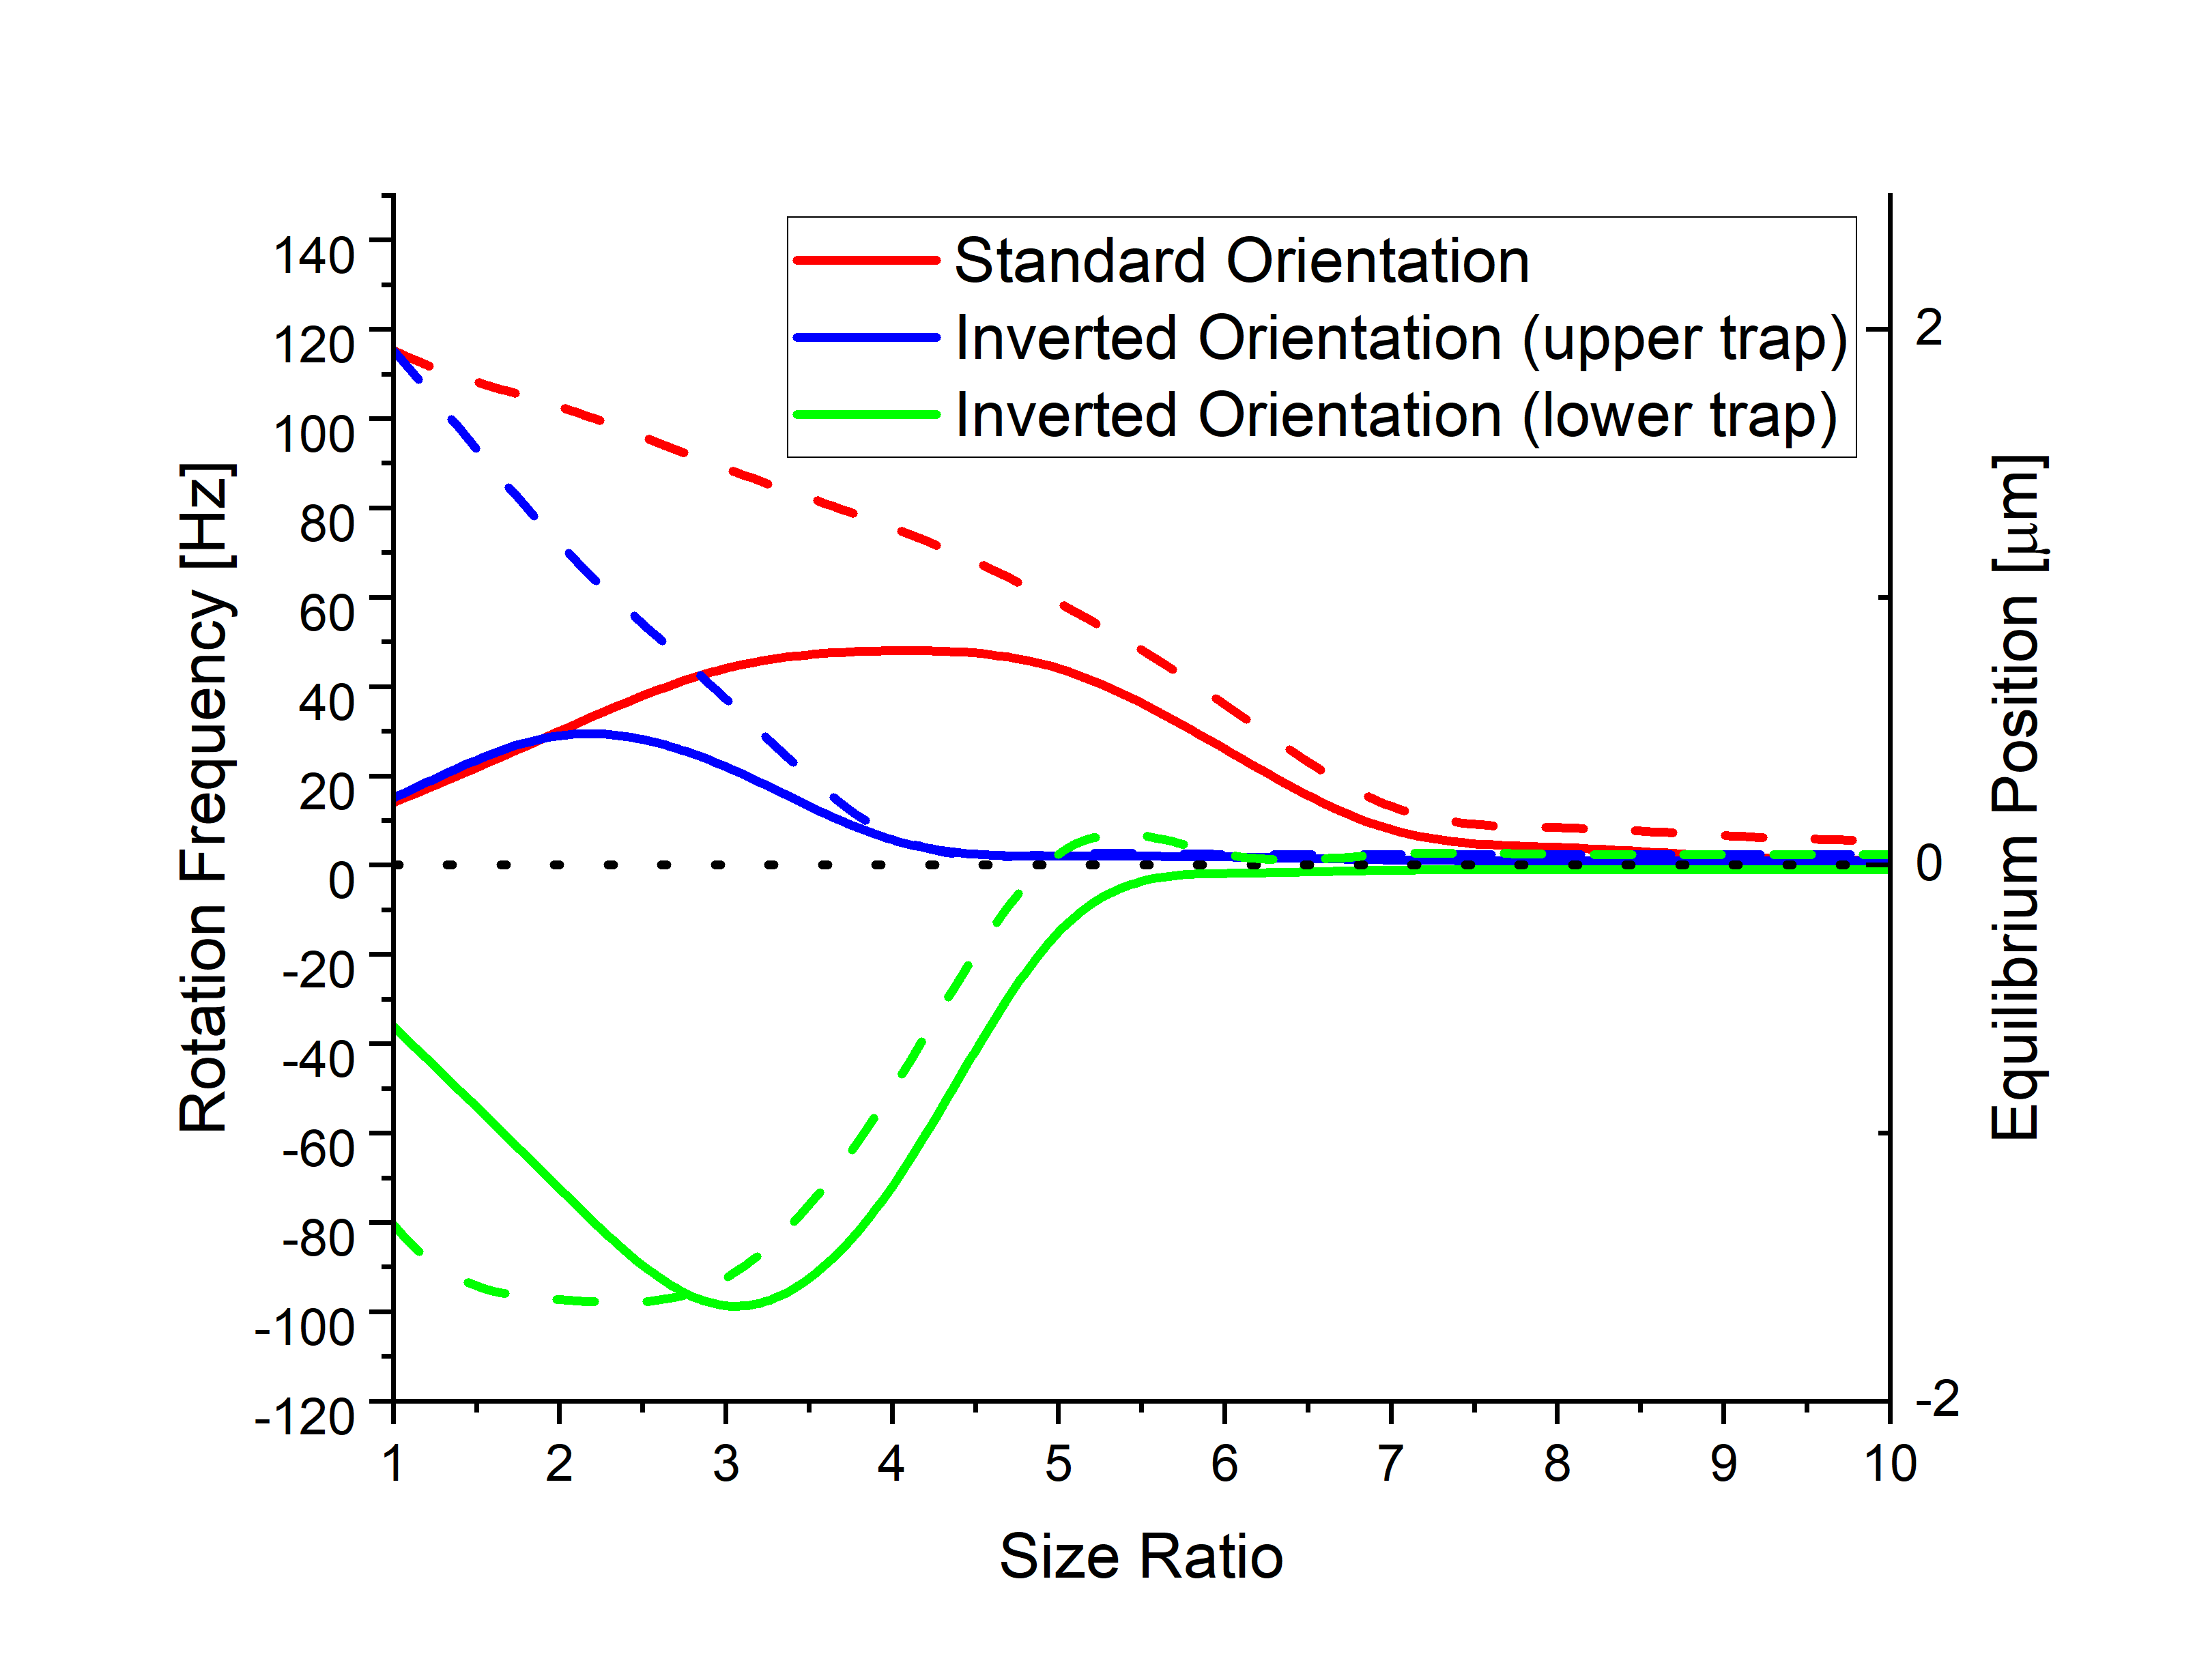
\includegraphics[width=0.65\linewidth]{rotation_rate_vs_size.png}
	\caption{Rotation rate plotted against dimer size ratio for a variety of different simulation scenarios. The red line is for the case where the larger sphere is above the smaller sphere. The blue line is the inverted case, while the initial position is above the focus of the trap. And lastly the green line is again for the inverted case, but when the dimer's initial position is below the focus of the trap.}
\end{figure}

Its difficult to see from the graph, but the rotation rate never truly goes down to zero, reaching a minimum of $~2\ Hz$, which would imply that a second sphere of radius $200\ nm$ is enough to induce rotational motion. These results are somewhat contrary to other work with silica dimers \cite{Ahn2018, Debuysschere2023}; previous experiments have trapped the dimer in an orientation perpendicular to the beam propagation direction. The rotational motion is induced due to the asymmetric geometry creating an unbalanced polarisation susceptibility along its long axis as compared to its short axis; therefore its long axis is aligned with the polarisation vector and can rotate freely\cite{Ahn2018}. This however cannot be the case with our simulations as the dimer rotates about its long axis, meaning there cannot be an asymmetric axis to align with the beam's polarisation vector. Furthermore because most of these experiments operate in the Rayleigh regime orientational effects are not usually considered whereas our own results make it clear that the initial orientation and position of spherical aggregates drastically effects their steady state behaviour.

\newpage

\section{Monitoring Stochastic rotational motion using static light scattering}
Orientational dynamics to an anisotropically scattering shape are difficult to characterise due to the coupling of rotational and translational effects. As shown in the previous chapter the dynamics of even simple dimers are heavily dependent on the particle's position and orientation, this is reflected in literature where several engineering solutions have been devised to decouple translational and orientational motion \textcolor{red}{[ , ]}. While a majority of latter work has been focused on nano-particles (falling into the Rayleigh Regime) and utilising florescence 

\subsection{Coordinate System}
In the case of our probe beam the +z direction points from the surface of the probe directly to the centre of diffusion in our dimer, with the +y direction pointing towards what would be our trapping beam, and the +x direction pointing into the page. The origin of our coordinate system is fixed on the centre of the focus of our trapping beam, meaning as our dimer's centre of diffusion moves the origin is kept constant.
\subsection{Dimer}
The dimer is defined by two spheres, in the trapping frame this would be orientated by $s=[0,0,1]$ however in our scattering set up this is rotated to $s=[-1,0,0]$ as the large sphere is furthest from the trapping beam. We scale the position of each sphere by the factor L:
\begin{align}
	L = \frac{1}{k} = \frac{\lambda}{2\pi}
\end{align}

Where $\lambda$ is the wavelength of light and is given in nanometres, this means every position must be also provided in nanometres.
\subsection{Beam}
Our probe beam is rather simple to define, we firstly say that the probe is a plane wave by setting the Gaussian beam parameter $C_B$ to 0. We also say the beam is un-polarized by defining the Stokes vector as $[1,0,0,0]$. 

\subsection{Detectors and Pixels}

Each detector is placed roughly $2\times 10^5 nm$ from the dimer (can be adjusted later for testing), with the position of the detector being defined by the polar and azimuth angles ($\theta$ \& $\phi$ respectively) such that:
\begin{align}
	[x_{fiber}, y_{fiber}, z_{fiber}] = [rcos(\phi)sin(\theta), rsin(\phi)sin(\theta), rcos(\theta)]
\end{align}
So if you were to place the fibers in the trapping frames x-y plane, in the probe beam frame will only have x and z components. The orientation of the detector is just the -ve of its position and not scaled by the distance term r, the orientation being the vector from the origin of the detector to the center of the dimer. 

Pixels can be thought of as points lying on the surface of the detector, by getting the spherical coordinates of each pixel we can compute the intensity at each point on the detector, allowing us to determine the average intensity on a given detector. The pixels are distributed using a sunflower distribution given by:

Where each point is first scaled to the size of the detector - for now we assume a radius of $2.5 \times 10^4 \ nm$ - and then translated from its position on the surface of the detector to the main coordinate system. Their orientation is treated much in the same as the detector's orientation, being its -ve position and scaled down by the radial distance from the dimer to the pixel, making it a unit vector. From their position we can also grab their spherical coordinates to create a list of points for mstm to evaluate. In order to accurately describe any detector surface we can use a Householder transformation to get the perpendicular circular surface of any vector.

This allows us to define the surface of any detector perpendicular to the origin of our coordinate system, we can freely choose the size and resolution of our fibre's. For every pixel we define the spherical coordinates relative to our origin, this is added to a list of $\theta, \phi$ pairs that are evaluated by MSTM. 

\section{Interpretation of scattering data into orientation estimates}
MSTM is capable of evaluating the scattering characteristics of a given target either in a fixed orientation or using an averaging of the particles orientation. While the latter method is satisfactory for simulation purposes it 


\bibliographystyle{ieeetran}
\bibliography{thesis_bib}

\end{document}